\documentclass[xcolor=table]{beamer}

\usepackage{booktabs}
\usepackage{hyperref}
\usepackage[table]{xcolor}
\usepackage{tikz}
\usepackage{graphics}
\usetikzlibrary{calc}

\setbeamertemplate{navigation symbols}{}%remove navigation symbols

\title{Finitely Repeated Games}
\subtitle{Game Theory}
\author{Vincent Knight}
\date{}

\begin{document}

\frame{\titlepage}

\frame{
$$
\Huge{
\begin{pmatrix}
(3,2)&(0,1)\\
(1,0)&(2,3)
\end{pmatrix}}
$$}

\frame{
$$
\begin{pmatrix}
(3,2)&(0,1)\\
(1,0)&(2,3)
\end{pmatrix}
$$
\begin{center}
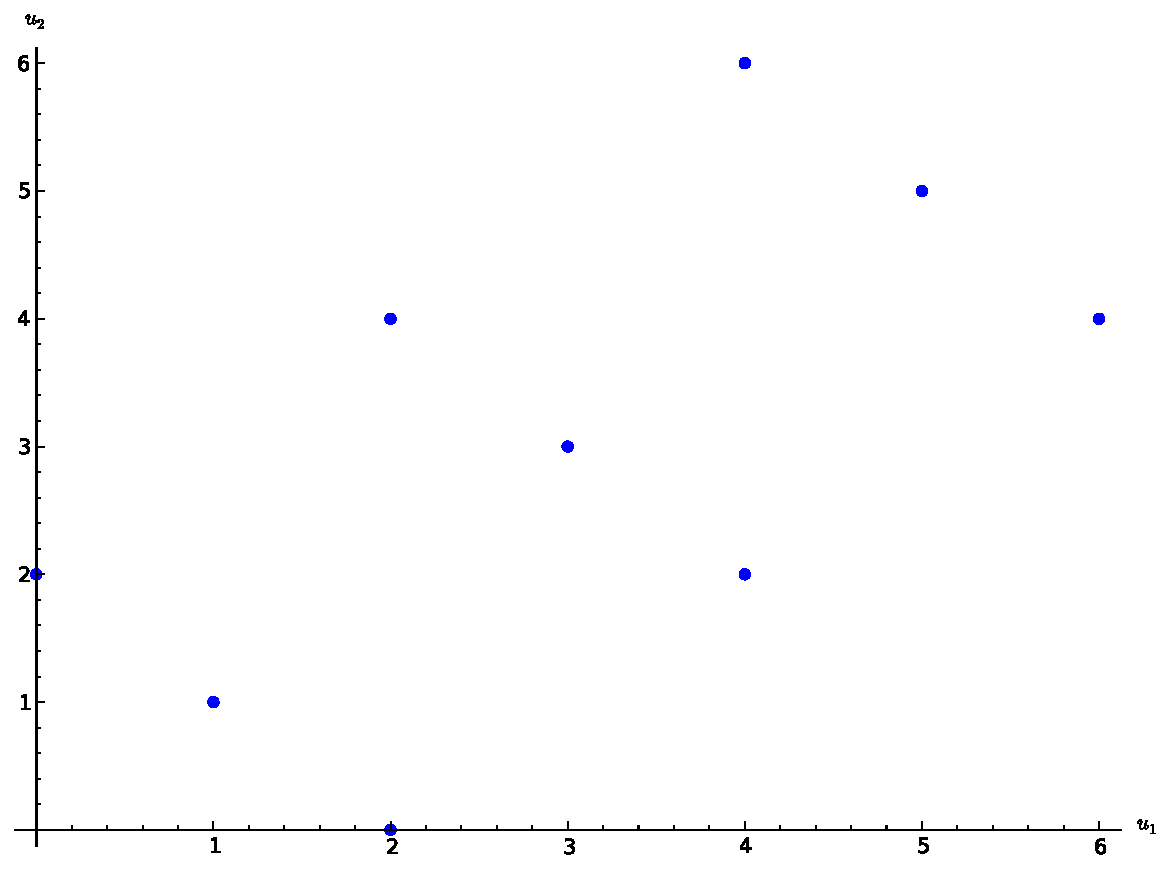
\includegraphics[width=.7\textwidth]{Images/twoshot.pdf}
\end{center}
}

\frame{
\textbf{A repeated game strategy must specify the action of a player in a given stage game given the entire history of the repeated game.}
\begin{center}
\pause
\textit{``Always player $r_1$.''}\\
\vspace{1cm}
\pause
\textit{``Player $r_2$ until opponent plays $s_1$, then play $r_1$.''}
\end{center}
}

\frame{
\textbf{Theorem.}
For any repeated game, any sequence of stage Nash profiles gives the outcome of a subgame perfect Nash equilibrium.

\pause
\begin{center}
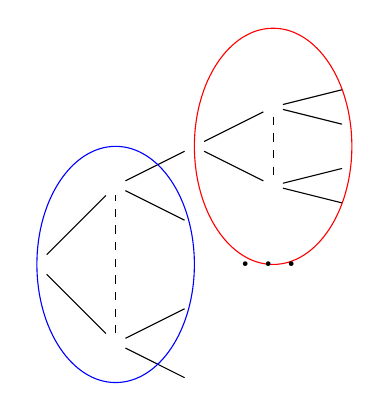
\begin{tikzpicture}
\node (A) at (0,0){};
\node (B) at (1,1){};
\node (C) at (1,-1){};
\node (D) at (2,1.5){};
\node (E) at (2,.5){};
\node (F) at (2,-.5){};
\node (G) at (2,-1.5){};
\node (H) at (3,2){};
\node (I) at (3,1){};
\node (J) at (4,2.25){};
\node (K) at (4,1.75){};
\node (L) at (4,1.25){};
\node (M) at (4,.75){};

\draw (A) -- (B);
\draw (A) -- (C);

\draw (B) -- (D);
\draw (B) -- (E);

\draw (C) -- (F);
\draw (C) -- (G);

\draw [dashed] (C) -- (B);

\draw (D) -- (H);
\draw (D) -- (I);

\draw [dashed] (H) -- (I);

\draw (H) -- (J);
\draw (H) -- (K);

\draw (I) -- (L);
\draw (I) -- (M);

\draw [blue] (1,0) ellipse (1cm and 1.5cm);
\draw [red] (3,1.5) ellipse (1cm and 1.5cm);

\node at (3,0) {\huge{\dots}};
\end{tikzpicture}
\end{center}

}


\end{document}
